%! Author = nico
%! Date = 23
\documentclass[a4paper, landscape, 8pt]{scrartcl}
\usepackage{csquotes}
\usepackage{subfiles}

% import template
% use german language
\usepackage[T1]{fontenc}
\usepackage[utf8]{inputenc}
\usepackage[english, ngerman]{babel}
\usepackage{lmodern}

% format
\usepackage{geometry}
\geometry{top=1.2cm, left=0.4cm, right=0.4cm}
\textheight = 550pt

% author
\usepackage{authblk}

% tables / tabular
\usepackage{tabularx}
\usepackage{makecell}
\usepackage{colortbl}

% math
\usepackage{amsmath}
\usepackage{amssymb}
\usepackage{amsfonts}
\usepackage{enumitem}

% graphic
\usepackage{graphicx}

% multi column
\usepackage{multicol}

%compact items
\setlist{topsep=0pt, leftmargin=4mm, nolistsep}
\setlength{\parindent}{0cm}

% header and footer
\usepackage{fancyhdr}
\pagestyle{fancy}

% header
\fancyhead[RO]{\AUTHOR | \INSTITUTE}
\fancyhead[LO]{\TITLE}

% footer
\fancyfoot[RO]{\CREATED}

\renewcommand\headrulewidth{0pt}
\renewcommand\footrulewidth{0pt}
\headsep = -2pt
\footskip = 0pt

% define Section format
\usepackage{sectsty}
\usepackage{titlesec}
\usepackage[dvipsnames]{xcolor}

\titleformat{name=\section}[block]{\sffamily\normalsize}{}{0pt}{\colorsection}
\titlespacing*{\section}{0pt}{0pt}{0pt}
\newcommand{\colorsection}[1]{%
	\colorbox{sectioncolor!80}{\parbox{0.98\linewidth}{\vspace{-1pt}\color{white}\ #1 \vspace{-2pt}}}}

% define Subsection format
\titleformat{name=\subsection}[block]{\sffamily\small}{}{0pt}{\colorsubsection}
\titlespacing*{\subsection}{0pt}{0pt}{0pt}
\newcommand{\colorsubsection}[1]{%
	\colorbox{subsectioncolor!80}{\parbox{0.98\linewidth}{\vspace{-1pt}\color{white}\ #1 \vspace{-2pt}}}}

% define SubSubsection format
\titleformat{name=\subsubsection}[block]{\sffamily\small}{}{0pt}{\colorsubsubsection}
\titlespacing*{\subsubsection}{0pt}{0pt}{0pt}
\newcommand{\colorsubsubsection}[1]{%
	\colorbox{subsubsectioncolor!60}{\parbox{0.98\linewidth}{\vspace{-1pt}\color{white}\ #1 \vspace{-2pt}}}}


% define colors
\definecolor{sectioncolor}{HTML}{191919}
\definecolor{subsectioncolor}{HTML}{0C5932}
\definecolor{subsubsectioncolor}{HTML}{0E693B}

\definecolor{b}{RGB}{0, 115, 192 } %Default highlight color
\definecolor{p}{RGB}{0, 43, 54} %Dark page color
\definecolor{t}{RGB}{131, 148, 150} %Dark text color

\definecolor{darkgreen}{RGB}{0,150,0}
\definecolor{dkgreen}{rgb}{0,0.6,0}
\definecolor{gray}{rgb}{0.5,0.5,0.5}
\definecolor{mauve}{rgb}{0.58,0,0.82}
\definecolor{DarkPurple}{rgb}{0.4, 0.1, 0.4}
\definecolor{DarkCyan}{rgb}{0.0, 0.5, 0.4}
\definecolor{LightLime}{rgb}{0.3, 0.5, 0.4}
\definecolor{Blue}{rgb}{0.0, 0.0, 1.0}
\definecolor{h}{RGB}{1, 101, 163}

% code listings
\usepackage{listings}
\usepackage{color}
\usepackage{beramono}
\usepackage{hyperref}
\hypersetup{
    colorlinks,
    linkcolor={black},
    citecolor={blue!50!black},
    urlcolor={blue!80!black}
}

\definecolor{bluekeywords}{rgb}{0,0,1}
\definecolor{greencomments}{rgb}{0,0.5,0}
\definecolor{redstrings}{rgb}{0.64,0.08,0.08}
\definecolor{xmlcomments}{rgb}{0.5,0.5,0.5}
\definecolor{types}{rgb}{0.17,0.57,0.68}

\definecolor{lstborder}{RGB}{24, 71, 21}
\definecolor{lstbackground}{RGB}{222, 230, 230}

\lstdefinestyle{eclipse-style}{
	frame=single,
	rulecolor=\color{lstborder},
	%backgroundcolor=\color{lstbackground},
	language=Java,
	showstringspaces=false,
	basicstyle=\ttfamily\scriptsize,
	keywordstyle=\color{RoyalBlue}\ttfamily,
    stringstyle=\color{darkgreen}\ttfamily,
	commentstyle=\color{DarkPurple!60}\ttfamily,
	identifierstyle=\color{black}\ttfamily,
	escapeinside={£}{£}, % latex scope within code
	breaklines=true,
	breakatwhitespace=true,
	showspaces=false,
	showtabs=false,
	tabsize=2,
	morekeywords={length},
	numberstyle=\tiny\color{darkgreen},
	aboveskip = 0em,
	belowskip = 0em,
	xleftmargin= 0em,
	framexleftmargin= 0em,
	gobble=20
}
\lstset{
	style=eclipse-style
	% literate=  % Allow for German characters in lstlistings.
	% {Ö}{{\"O}}1
	% {Ä}{{\"A}}1
	% {Ü}{{\"U}}1
	% {ü}{{\"u}}1
	% {ä}{{\"a}}1
	% {ö}{{\"o}}1}
}

% creation date
\usepackage{filemod}
\newcommand{\CREATED}{\filemodprintdate{\jobname}}

% front page
\newcommand{\AUTHOR}{Nico Fehr }
\newcommand{\INSTITUTE}{Ostschweizer Fachhochschule}

% no indentation
\setlength{\parindent}{0cm}

% new item tabitem for bullet points in tables
\newcommand{\tabitem}{~~\llap{\textbullet}~~}

\usepackage[ngerman]{babel}


% document information
\newcommand{\SUBJECT}{}
\newcommand{\TITLE}{Cheat sheet für Data Engineering (DatEng)}

% document content
\begin{document}

    \begin{multicols*}{4}
        \setlength{\columnseprule}{0.4pt}
        \footnotesize

        \section{Objekt-Relationale Mapper (O/R-Mapper)}
        Ziel: Semantische Lücke schliessen.
        Programme sind meist objektorientiert, DBs meist relational.

        \subsection{OR-Mapping Varianten}
        \begin{enumerate}
            \item Forward Engineering (Code first, Top-Down)
            \subitem Business-Modell erstellen, erzeuge DB-Schema
            \item Bottom Up (DB first, \enquote{Reverse Engineering})
            \subitem DB-Schema existiert, erzeuge Business-Modell
            \item Inside-Out (Mapping first)
            \subitem Erstelle Metadaten, generiere Java und DB-Schema
            \item Meet-in-the-middle (Outside-in)
            \subitem Business-Modell und DB-Schema existieren, erstelle Metadaten
            \item Meta Model (Model-driven)
        \end{enumerate}

        \subsection{JPA Layers}
        \begin{tabular}{l | l}
            \cellcolor{darkgreen!25} Java Program & Appl. mit persistenten Objekten \\
            \hline
            \cellcolor{Blue!25} JPA (Core) & Standard ORM Interface (JEE) \\
            \hline
            \cellcolor{darkgreen!25} JPA Provider & JPA Implementierung (Third Party) \\
            \hline
            \cellcolor{Blue!25} JDBC API & Standard JDBC Interface \\
            \hline
            \cellcolor{darkgreen!25} JDBC Driver & JDBC Driver (Third Party) \\
            \hline
            \cellcolor{gray!25} Database &
        \end{tabular}

        \subsection{Entity-Klassen}
        Können:
        \begin{itemize}
            \item erben, vererben
            \item interfaces implementieren
            \item abstract sein
        \end{itemize}
        Beispiel:
        \begin{lstlisting}[language=java]
                    @Entity
                    @Table(name = "account")
                    public class BankAccount {
                        @Id
                        @Column(name = "accountId")
                        private long id;
                        private double balance;
                        @Column(name = "salary", scale=10, precision=2)
                        private BigDecimal salary;
                        @Column(name = "description", length=500)
                        private String explanation;
                        @Temporal(TemporalType.TIMESTAMP)
                        private Calendar creationDate;
                        @Column(name = "s_time", columnDefinition="TIMESTAMPZ")
                        private Calendar startDate;
                        @Enumerated(EnumType.STRING)
                        private Currency curr;
                        @Column(name = "ssn", unique=true, nullable=true)
                        private long ssn;
                        @Transient
                        private String tempComments;
                        // getter und setter
                    }
        \end{lstlisting}

        \subsection{Laden/Suchen von Entities}
        \begin{lstlisting}[language=java]
                    EntityManagerFactory factory = Persistence.createEntityManagerFactory("Bank");
                    EntityManager em = factory.createEntityManager();
                    Query query = em.createQuery("SELECT a FROM BankAccount a");
                    List<BankAccount> list = query.getResultList();
                    for (BankAccount account : list) {
                        System.out.println(account);
                    }
                    em.close();
        \end{lstlisting}

        \subsection{Insert von Entities \tiny{Explizit}}
        \begin{lstlisting}[language=java]
                    EntityManager em = factory.createEntityManager();
                    em.getTransaction().begin();
                    BankAccount account = new BankAccount();
                    account.setName("Bill");
                    em.persist(account);
                    em.getTransaction().commit();
                    em.close();
        \end{lstlisting}

        \subsection{Updates / Delete von Entities}
        \begin{lstlisting}[language=java]
                    EntityManager em = factory.createEntityManager();
                    em.getTransaction().begin();
                    BankAccount account = em.find(BankAccount.class, 1L);

                    // Update
                        account.incBalance(100);

                    // Delete
                        em.remove(account);
                    em.getTransaction().commit();
        \end{lstlisting}

        \subsubsection{Mapping in XML}
        Priorität Mapping
        \begin{enumerate}
            \item Mapping-File \enquote{orm.xml}
            \item Entity Annotationen
            \item Default Mapping (in JPA-Implementation)
        \end{enumerate}

        \subsection{JPA Lifecycle}
        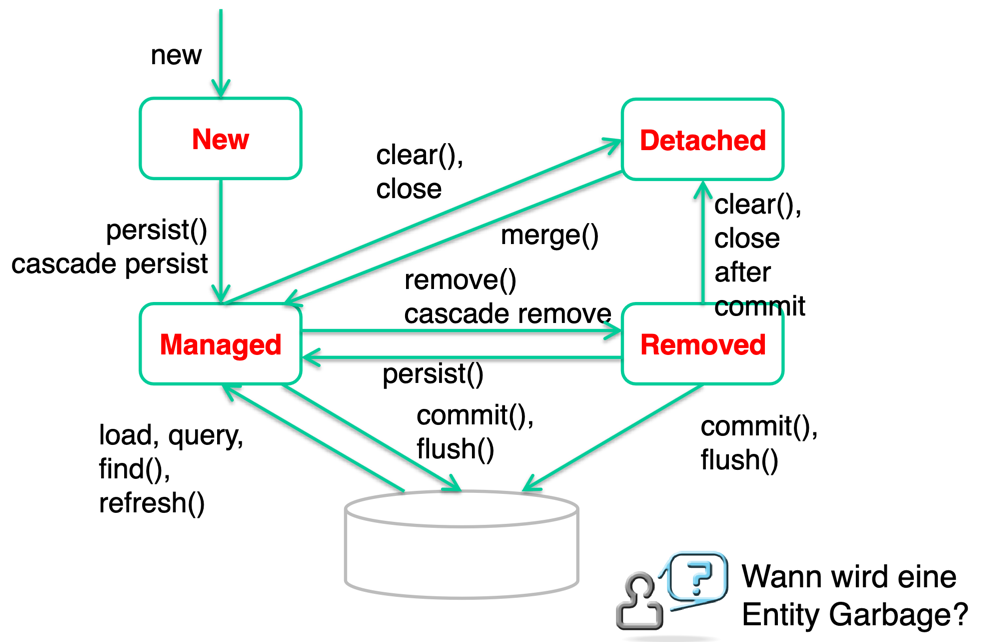
\includegraphics[scale=0.12]{graphic/00-entity-lifecycle}

        \subsection{JPA Architektur}
        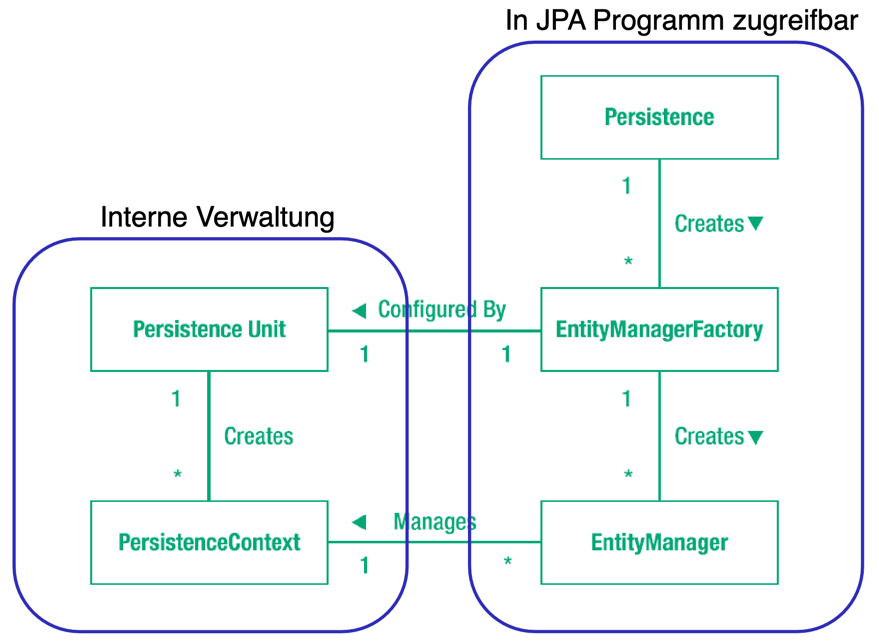
\includegraphics[scale=0.12]{graphic/01-jpa-architecture}

        \subsection{Entity States}
        Entitätsinstanzen befinden sich in einem von 4 Zuständen: \\
        \begin{tabularx}{\columnwidth}{l | X}
            \hline
            New & keine persistente Identität, noch nicht mit Persistenzkontext verbunden\\
            \hline
            Managed & Entitätsinstanzen haben persistente Identität und sind mit Kontext verknüpft\\
            \hline
            Detached & Losgelöste Entitätsinstanzen haben Identität und sind derzeit nicht mit Kontext verbunden\\
            \hline
            Removed & Entfernte Instanzen haben Identität, sind mit Kontext verknüpft und sind für Entfernung aus Datenspeicher vorgesehen
        \end{tabularx}

        \subsection{JPA Transaktionen}
        \begin{lstlisting}[language=java]
                    // Explizite Transaktion
                    EntityManager em = factory.createEntityManager();
                    em.getTransaction().begin();
                    // do stuff
                    em.getTransaction().commit(); // or rollback();
        \end{lstlisting}

        \subsubsection{Transaction Isolation}
        JPA basiert auf READ COMMITED isolation level.
        JPA Provider EclipseLink führt Reads nicht über gleiche Connection wie Write aus.

        \begin{lstlisting}[language=java]
                    // Explizites Locking
                    BankAccount account = em.find(...);
                    em.lock(account, LockModeType.PESSIMISTIC_WRITE);
                    account.incBalance(100);
        \end{lstlisting}

        \subsection{Object Identity}
        \begin{itemize}
            \item Session (=Instanz EntityManager, =Persistence Context) übersetzt DB Konzept von Primärschlüssel in Konzept von Objekt-Instanzen
            \item Session verwaltet Objekt Identität
            \subitem Objekte über Id im Cache verwaltet
            \subitem Bei 1. Zugriff wird Objekt aus DB geladen, bei weiteren, Kopie aus dem Cache
            \subitem Persistente Objekte identifiziert über DB-Identität
        \end{itemize}

        \subsubsection{Entity-Identität}
        \begin{itemize}
            \item Annotation @Id, Generierung der Identity mit @GeneratedValue
            \item Verschiedene Strategien
            \subitem AUTO: von JPA Provider gewählt (meist SEQUENCE, IDENTITY)
            \subitem IDENTITY: basiert auf \enquote{auto-increment} (GENERATED AS...) Wert der DB
            \subitem SEQUENCE: basiert auf SEQUENCE DB-Objekt
            \subitem TABLE: basiert auf explizierter Primary-Key DB-Tabelle (selten)
        \end{itemize}

        \subsection{Generierungstypen}
        \subsubsection{Identity}
        \begin{lstlisting}[language=java]
                    @Id
                    @GeneratedValue(strategy = GenerationType.IDENTITY)
                    private long accountId;
        \end{lstlisting}
        \begin{lstlisting}[language=sql]
                    CREATE TABLE bankaccount (
                        accountid GENERATED ALWAYS AS IDENTY NOT NULL, -- frueher SERIAL in PostgreSQL
                        CONSTRAINT account_pkey PRIMARY KEY (accountid)
                        ...
                    )
        \end{lstlisting}

        \subsubsection{Sequence}
        \begin{lstlisting}[language=java]
                    @Id
                    @GeneratedValue(strategy = GenerationType.SEQUENCE, generator = "BankCustGen")
                    @SequenceGenerator(name = "BankCustGen",
                                       sequenceName = "customeridseq",
                                       allocationSize = 1)
                    // nur einmal ausfuehren
                    private long customerId;
        \end{lstlisting}
        \begin{lstlisting}[language=sql]
                    -- explizites sequence Objekt in DB
                    CREATE SEQUENCE customeridseq;
        \end{lstlisting}

        \subsubsection{Table}
        \begin{lstlisting}[language=java]
                    @Id
                    @GeneratedValue(strategy = GenerationType.TABLE,
                        generator = "CustomerGen")
                    @TableGenerator(name = "CustomerGen", table = "keytable",
                        pkColumnName = "keyname",
                        valueColumnName = "keyvalue",
                        pkColumnValue = "customerkey")
                    private long customerId;
        \end{lstlisting}

        \textbf{keytable} (Tabelle zur Key-Verwaltung)\\
        \begin{tabularx}{\columnwidth}{l | X}
            \textbf{keyname} & \textbf{keyvalue} \\
            \hline
            customerkey & 100 \\
            \hline
            accountkey & 3214
        \end{tabularx}

        \subsection{Bidirektionalität}
        \subsubsection{Inkonsistenz}
        Bidirektionale Relationen sind bei Änderungen durch JPA nicht synchronisiert.
        \begin{itemize}
            \item Trotz Angabe von \texttt{@OneToMany(mappedBy="customer")}
            \item Nur nach Laden konsistent
        \end{itemize}

        \subsection{OneToOne (1:1)}
        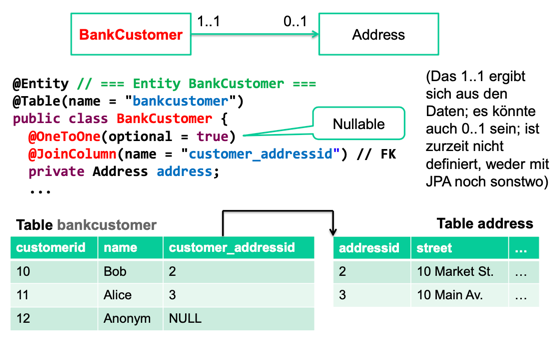
\includegraphics[scale=0.25]{graphic/02-one-to-one}
        \subsubsection{Bidirectional}
        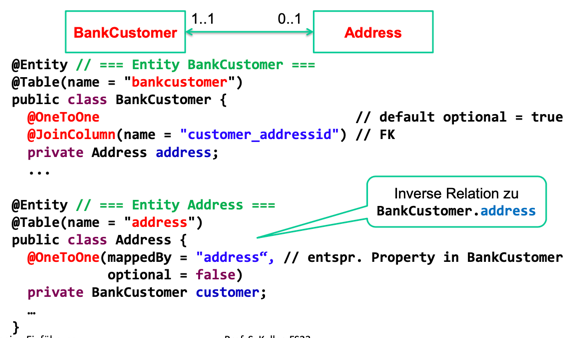
\includegraphics[scale=0.25]{graphic/03-bidirectional-one-to-one}
        \subsubsection{Inverse}
        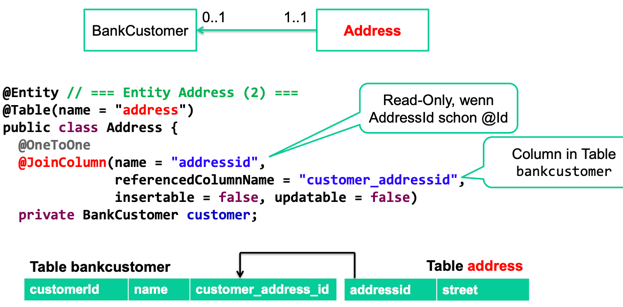
\includegraphics[scale=0.25]{graphic/04-inverse-one-to-one}

        \subsection{ManyToOne (Many:1)}
        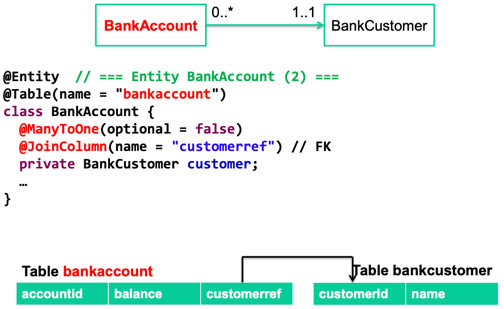
\includegraphics[scale=0.25]{graphic/05-many-to-one}
        \subsubsection{Bidirectional}
        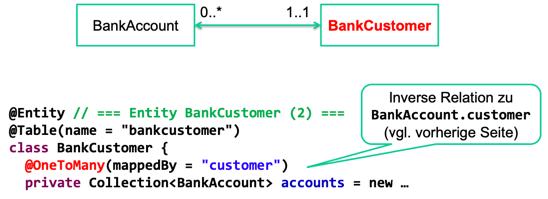
\includegraphics[scale=0.25]{graphic/06-bidirectional-many-to-one}

        \subsection{OneToMany (1:Many)}
        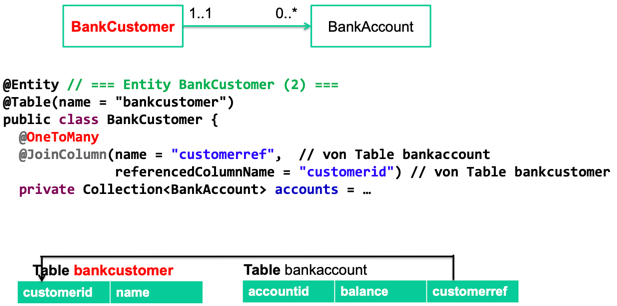
\includegraphics[scale=0.25]{graphic/07-one-to-many}

        \subsection{ManyToMany (Many:Many)}
        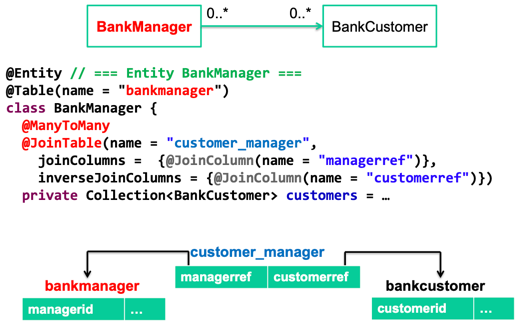
\includegraphics[scale=0.25]{graphic/08-many-to-many}
        \subsubsection{Bidirectional}
        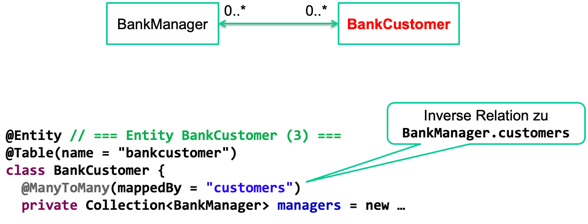
\includegraphics[scale=0.25]{graphic/09-bidirectional-many-to-many}
        
        \subsection{Ladestrategien}
        \begin{itemize}
            \item \texttt{@OneToOne(fetch = FetchType.LAZY)}
            \subitem Default bei \texttt{@OneToMany} und \texttt{@ManyToMany}
            \item \texttt{@OneToMany(fetch = FetchType.EAGER)}
            \subitem Default bei \texttt{@OneToOne} und \texttt{@ManyToOne}
        \end{itemize}

        \subsection{Kaskadieren}
        \begin{lstlisting}[language=java]
                    // Cascade.Persist
                    @OneToMany(cascade = CascadeType.PERSIST, ...)
                    // CascadeType.Remove
                    @OneToMany(cascade = CascadeType.REMOVE)
                    private Collection<BankAccount> accounts = new ArrayList<>();
        \end{lstlisting}
        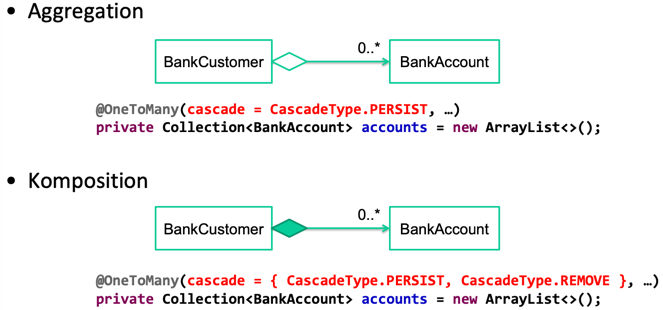
\includegraphics[scale=0.24]{graphic/10-relations-with-dependencies}

        \subsection{Bidirectional Sync}
        Bidirektionale Relationen sind bei Änderungen durch JPA nicht synchronisiert.
        \begin{lstlisting}[language=java]
                    public class BankAccount {
                        ...
                        public void setCustomer(BankCustomer newCustomer) {
                            BankCustomer oldCustomer = this.customer;
                            this.customer = newCustomer;
                            if (newCustomer != null && !newCustomer.containsAccount(this)) {
                                newCustomer.addAccount(this);
                            }
                            if (oldCustomer != null && oldCustomer.containsAccount(this)) {
                                oldCustomer.removeAccount(this);
                            }
                        }
                    }
                    ...
                    public class BankCustomer {
                        ...
                        public void addAccount(BankAccount account) {
                            this.accounts.add(account);
                            if (account.getCustomer() != this) {
                                account.setCustomer(this);
                            }
                        }
                    }
        \end{lstlisting}

        \subsection{Vererbung: Abbildungsstrategien}
        \begin{tabularx}{\columnwidth}{l | X}
            SINGLE TABLE & Einzige Tabelle für Superklasse (+ type); JPA Default. (3c) \\
            \hline
            JOINED TABLE & Je Tabelle pro Sub- und Superklasse (+ type + Beziehungen). (3a, \enquote{Tabelle pro Klasse}) \\
            \hline
            TABLE PER CLASS & Je Tabelle pro Klasse (inkl. vererbte Columns), d.h. mit redundanten Columns (3b, hatte keine Superklasse) \\
            \hline
            MAPPED SUPERCLASS & Je Tabelle pro Klasse (inkl. vererbte Columns). Ähnlich wie TABLE PER CLASS aber ohne Superklasse. (3b)
        \end{tabularx}

        \subsubsection{Single Table}
        \begin{lstlisting}[language=java]
                    @Entity
                    @Inheritance(strategy = InheritanceType.SINGLE_TABLE)
                    @DiscriminatorColumn(name = "type")
                    public abstract class BankCustomer {
                        @Id private String name;
                    }
                    ...
                    @Entity
                    @DiscriminatorValue("Retail")
                    public class RetailBankCustomer extends BankCustomer {
                        private int fees;
                    }
                    ...
                    @Entity
                    @DiscriminatorValue("Private")
                    public class PrivateBankCustomer extends BankCustomer {
                        private String eliteOffer;x
                    }
        \end{lstlisting}

        \subsubsection{Joined Table}
        Eine Tabelle \texttt{bankcustomer}.
        Zwei Tabellen \texttt{retailbankcustomer} und \texttt{privatebankcustomer} mit FK auf \texttt{bankcustomer}.
        \begin{lstlisting}[language=java]
                    @Entity
                    @Inheritance(strategy = InheritanceType.JOINED)
                    @DiscriminatorColumn(name = "type")
                    public abstract class BankCustomer {
                        @Id private int customerId;
                        private String name;
                    }
                    ...
                    @Entity
                    @DiscriminatorValue("Retail")
                    public class RetailBankCustomer extends BankCustomer {
                        private int fees;
                    }
                    ...
                    @Entity
                    @DiscriminatorValue("Private")
                    public class PrivateBankCustomer extends BankCustomer {
                        private String eliteOffer;
                    }
        \end{lstlisting}
        
        \subsubsection{Table per Class}
        \begin{lstlisting}[language=java]
                    @Entity
                    @Inheritance(strategy = InheritanceType.TABLE_PER_CLASS)
                    public abstract class BankCustomer {
                        @Id
                        private int customerId;
                        private String name;
                    }
                    ...
                    @Entity
                    public class RetailBankCustomer extends BankCustomer {
                        private int fees;
                    }
                    ...
                    @Entity
                    public class PrivateBankCustomer extends BankCustomer {
                        private String eliteOffer;
                    }
        \end{lstlisting}

        \section{JPQL \tiny{Java Persistence Query Language}}
        \subsection{Query Parameters}
        \begin{tabularx}{\columnwidth}{l | X}
            Positional & \texttt{select a from BankAccount a where a.customer.name like \textcolor{red}{?1} and a.balance >= \textcolor{red}{?2}} \\
            \hline
            Named & \texttt{select a from BankAccount a where a.customer.name like \textcolor{red}{:name} and a.balance >= \textcolor{red}{:lower}}
        \end{tabularx}

        \subsection{Criteria API}

        \subsection{Weitere Beispiele}


        \section{Stored Procedures}
        Synonyme: User Defined Functions, Subroutine, Methode.

        \begin{tabularx}{\columnwidth}{l | X}
            Vorteile & \tabitem Domänen Logik (Funktionen, Datenkapselung) \\
            & \tabitem Performanz: Funktionen nahe bei Daten \\
            & \tabitem Triggers \\
            & \tabitem Konsistenz: Triggers Security (GRANT auf SP, Log auditing) \\
            & \tabitem Separation of Concern/Duties sowie Wiederverwendbarkeit des Codes \\
            \hline
            Nachteile & \tabitem Manchmal reichen Views \\
            & \tabitem Manchmal reichen ORM (Object-Relational Mapper) \\
            & \tabitem Macht Software-Entwicklungsprozess komplizierter \\
            & \tabitem Portierbarkeit
        \end{tabularx}

        \subsection{Syntax}
        \begin{lstlisting}[language=sql]
                    create [or replace] [function | procedure] name ( [ [argname] argtype [,...] ] )
                        [ returns rettype | returns setof record ]
                    language [plpgsql | SQL | ...] [optimizers]
                    as $$
                      -- ... Source Code gemaess "language"
                    $$;
                    drop function name(argtype [,...]);
        \end{lstlisting}

        \section{PL/pgSQL \tiny{Prozedurale Sprache von PostgreSQL}}
        Hello World / Dynamisches SQL: \\
        \begin{lstlisting}[language=sql]
                    -- Hello World
                    create or replace
                    -- function helloworld()
                    -- returns void
                    -- besser new style pl/sql-kompatibel
                    procedure helloworld()
                    language plpgsql as $$
                    declare
                        result int;
                    begin
                       raise notice 'Hello World!';
                       -- dynamisches sql
                       execute 'SELECT 1' into result;
                    end;
                    $$;
                    -- Test and use the function/procedure:
                    select helloworld();
        \end{lstlisting}

        PL/pgSQL mit Parameter: \\
        \begin{lstlisting}[language=sql]
                    create or replace function
                      pow_mod(bigx bigint, n bigint, m bigint)
                    returns bigint
                    /*
                        -- tabelle zurueckgeben
                        RETURNS TABLE (
                            abtname VARCHAR,
                            abtMA VARCHAR
                        )
                    */
                    as $$
                    declare
                      x bigint;
                      xx bigint;
                    begin
                      if n = 0 then return 1; end if;
                      x := bigx % m;
                      xx := (x * x) % m;
                      if n % 2 = 0 then
                        return pow_mod(xx, n/2, m);
                      else
                        return (x * pow_mod(xx, (n-1)/2, m)) % m;
                      end if;
                    end;
                    $$ language plpgsql;
        \end{lstlisting}

        Set Returning Functions \\
        \begin{lstlisting}[language=sql]
                    CREATE OR REPLACE FUNCTION getAllFoo() RETURNS SETOF foo AS $$
                        DECLARE
                              r foo%rowtype;  -- Tabelle foo
                        BEGIN
                            FOR r IN SELECT * FROM foo WHERE fooid > 0
                            LOOP
                                -- do something...
                                RETURN NEXT r; -- return current row of SELECT
                            END LOOP;
                            RETURN; -- generic return
                        END
                    $$ LANGUAGE 'plpgsql';
        \end{lstlisting}

        SPs ausführen:
        \begin{itemize}
            \item \texttt{perform <<...>>};
            \item \texttt{do \$\$<<Anonymous code block>>\$\$;}
        \end{itemize}

        \subsection{SP Compiler}
        \begin{enumerate}
            \item Code wird beim Aufruf geparsed
            \item als Pseudocode in der DB gespeichert
            \item bei der ersten Ausführung wird volle Syntax gecheckt
            \item SQLStatements werden vorkompiliert (wie JDBC PreparedStatement) und bei wiederholtem Aufruf wiederverwendet.
            \item Code läuft im Server ab
            \item Kommunikation mit Frontend über Rückgabewerte (SP ungeeignet für GUI)
        \end{enumerate}

        \subsection{Cursor}
        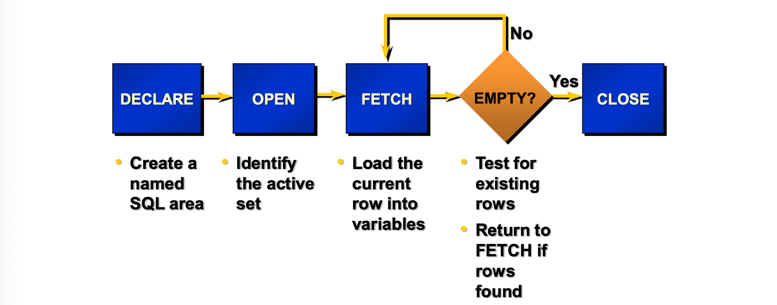
\includegraphics[width=\columnwidth]{graphic/15-cursor-process}

        \begin{lstlisting}[language=sql]
                    CREATE OR REPLACE
                    FUNCTION BerechneSalSumme (ChefPersNr Angestellter.PersNr%TYPE)
                    RETURNS DECIMAL AS $$
                        DECLARE
                           AngCursor refcursor; -- cursor variable unbound
                           SalSumme DECIMAL (10, 2) := 0;
                           AngRec RECORD;
                        BEGIN
                        OPEN AngCursor FOR SELECT Ang.PersNr,Ang.Name,Ang.Salaer
                                             FROM Angestellter Ang
                                             WHERE Ang.Chef = ChefPersNr;
                          LOOP /*Iteration ueber Resultatmenge*/
                            FETCH AngCursor INTO AngRec;
                            EXIT WHEN NOT FOUND;
                            SalSumme := SalSumme + AngRec.Salaer;
                            SalSumme := SalSumme + BerechneSalSumme (AngRec.PersNr); //Rekursion
                          END LOOP;
                          CLOSE AngCursor;
                          RETURN SalSumme;
                        END;
                    $$ language plpgsql;
                    select BerechneSalSumme(1001);
        \end{lstlisting}

        \subsubsection{Cursor for Update}


        \section{Triggers}
        \begin{itemize}
            \item Implementation von komplexen Konsistenzbedingungen
            \item Sicherheit, z.B. wenn Änderungen nur während Arbeitstagen ausgeführt werden können
            \item Berechnen von abgeleiteten Attributen
            \item Sammlen von Statistik- und Logdaten
            \item DB-Objekte $\to$ immer einer Tabelle zugeordnet
            \item in SP programmiert, namentlich als PL/pgSQL-Function
            \item haben keine Funktions-Parameter
            \item können nicht direkt aufgerufen werden
            \item werden vom DBMS beim Eintreten eines \enquote{DB-Events} aufgerufen
            \item haben bei Ausführung die Rechte ihres Owners
        \end{itemize}

        \subsection{Syntax}
        \begin{lstlisting}[language=sql]
                    DECLARE
                        -- optional
                    BEGIN
                        -- executable part
                    EXCEPTION
                        -- optional
                        /* Multi line comments */
                    END;

                    -- Jedes objekt kann auch DESCRIPTION haben:
                    COMMENT ON FUNCTION increment(int) is 'Increment 1';
        \end{lstlisting}

        \subsection{Spezielle Deklarationen}
        \begin{lstlisting}[language=sql]
                    DECLARE
                        var5 angestellter.id%TYPE; --int
                        var6 angestellter%ROWTYPE;
                        var7 RECORD;
                    ...
        \end{lstlisting}

        \subsection{Trigger-Funktions-Variablen}
        \begin{tabularx}{\columnwidth}{l | X}
            \textbf{TG\_NAME} & Name von Trigger \\
            \hline
            \textbf{TG\_WHEN} & BEFORE / AFTER \\
            \hline
            \textbf{TG\_LEVEL} & ROW / STATEMENT \\
            \hline
            \textbf{TG\_OP} & INSERT, UPDATE, DELETE, TRUNCATE \\
            \hline
            \textbf{TG\_RELID} & ROW ID der Tabelle \\
            \hline
            \textbf{TG\_RELNAME} & Name der Tabelle \\
            \hline
            \textbf{TG\_TABLE\_SCHEMA} & Schema der Tabelle \\
            \hline
            \textbf{NEW, OLD} & neue / alte Records
        \end{tabularx}

        \subsection{Auditing mit Triggers}
        \begin{lstlisting}[language=sql]
                    CREATE TABLE ang_audit(
                        operation char(1)   NOT NULL,
                        stamp timestamp NOT NULL,
                        userid text      NOT NULL,
                        angname text      NOT NULL,
                        salaer integer
                    );

                    CREATE TRIGGER ang_audit
                    AFTER INSERT OR UPDATE OR DELETE ON Angestellter
                    FOR EACH ROW
                    EXECUTE PROCEDURE process_ang_audit();

                    CREATE OR REPLACE FUNCTION process_ang_audit()
                    RETURNS TRIGGER AS $$
                        BEGIN
                            IF (TG_OP = 'DELETE') THEN
                                INSERT INTO ang_audit
                                SELECT 'D', now(), user, OLD.name, OLD.salaer;
                                RETURN OLD;
                            ELSIF (TG_OP = 'UPDATE') THEN
                                INSERT INTO ang_audit
                                SELECT 'U', now(), user, NEW.name, NEW.salaer;
                            ELSIF (TG_OP = 'INSERT') THEN
                                INSERT INTO ang_audit
                                SELECT 'I', now(), user, NEW.name, NEW.salaer;
                            END IF;
                            RETURN NULL; -- result ignored => AFTER trigger
                        END;
                    $$ language plpgsql;
        \end{lstlisting}

        \subsection{Ausschalten}
        \begin{lstlisting}[language=sql]
                    ALTER TABLE mytable DISABLE TRIGGER mytrigger | ALL;
        \end{lstlisting}

        \section{Updatable Views}
        \begin{lstlisting}[language=sql]
                    CREATE VIEW myview AS SELECT ...
        \end{lstlisting}
        \textbf{Updatable Views erstellen mit:}
        \begin{itemize}
            \item Stored Procedures
            \item Updatable Views - automatisch aktualisierbare Views
            \subitem automatisch aktualisierbare Views
            \subitem nur möglich, wenn bestimmte Bedingungen erfüllt
            \item Instead of-Triggers
        \end{itemize}

        \textbf{Views sind automatisch aktualisierbar wenn:}
        \begin{itemize}
            \item Genau einen Eintrag in der FROM-Klausel (andere Tabelle oder andere updatable View)
            \item Keine WITH, DISTINCT, GROUP BY, HAVING, LIMIT, OFFSET
            \item kein UNION, INTERSECT, EXCEPT
            \item SELECT-Liste besitzt keine Aggregation, Window-Funktion oder SET-Returning-Funktion
        \end{itemize}

        \subsection{Instead of-Triggers}
        Nur für Views und nicht für Tabelle möglich.
        Leiten Modifikation (INSERT, UPDATE, DELETE) auf Views zur darunterliegenden Tabelle weiter.

        \begin{lstlisting}[language=sql]
                    --DROP FUNCTION IF EXISTS abtleiterinfo_update_abtchef_fn() CASCADE;
                    CREATE OR REPLACE FUNCTION abtleiterinfo_update_abtchef_fn()
                    RETURNS TRIGGER AS $$
                        BEGIN
                            IF TG_OP = 'UPDATE' THEN
                                UPDATE abtleitung SET abtchef=NEW.abtchef WHERE abtnr=OLD.abtnr;
                                RETURN NEW; -- New Record ist resultset
                            END IF;
                        END;
                    $$ LANGUAGE plpgsql;

                    CREATE TRIGGER abtleiterinfo_update_abtchef
                        INSTEAD OF UPDATE ON abtleiterinfo
                        FOR EACH ROW
                        EXECUTE PROCEDURE abtleiterinfo_update_abtchef_fn();

                    UPDATE abtleiterinfo SET abtchef=1019 WHERE abtnr=2; -- is possible now
        \end{lstlisting}

        \section{Materialized Views}
        \begin{lstlisting}[language=sql]
                    -- create materialized view (snapshot)
                    CREATE MATERIALIZED VIEW myMatView as SELECT ...

                    -- refresh materialized view
                    REFRESH MATERIALIZED VIEW myMatView;

                    -- refresh materialized view concurrently (view is available during updates)
                    REFRESH MATERIALIZED VIEW CONCURRENTLY myMatView;
        \end{lstlisting}

        \begin{tabularx}{\columnwidth}{l X}
            Snapshot & updated once (REFRESH in PostgreSQL) \\
            \hline
            Eager & updates as underlying table is updated \\
            \hline
            Lazy & updated when transaction commits \\
            \hline
            Andere & Oracle: \enquote{User defined}, \enquote{Per Interval}
        \end{tabularx}

        \subsection{Temporäre Tabellen}
        Tabelle wird automatisch am Ende der Transaktion oder Session gelöscht.
        \begin{lstlisting}[language=sql]
                    CREATE TEMPORARY TABLE tmp AS SELECT ...
        \end{lstlisting}

        \section{Datentyp}
        \subsection{Abstrakter Datentyp {\tiny ADT}}
        Datentyp, der durch Operationen definiert ist, Zugriff und Verwaltung zu ermöglichen und realisieren.
        HINWEIS: ADT kann ADT enthalten, z.B. Stack als Liste.
        Bestandteile:
        \begin{tabularx}{\columnwidth}{l | X}
            \textbf{Datentyp ADT} & \textbf{Beispiel} \\
            \hline
            Name & \texttt{easteregg} \\
            \hline
            Innere Datenstruktur & \texttt{outer: text, inner: text;} \\
            \hline
            Konstruktor & \texttt{easteregg\_from\_text('x', 'yy')} \\
            \hline
            Accessor-Funktion & \texttt{easteregg\_inner()} \\
            \hline
            Update-Funktion & \texttt{easteregg\_append('zz')} \\
            \hline
            Hilfs-Funktion & \texttt{easteregg\_astext(myegg)} \\
            \hline
            Operator & \texttt{WHERE myegg = youregg} \\
            \hline
            Index auf Attribut \texttt{eggs} & \texttt{CREATE INDEX myindex ON mytable USING GIN(eggs);}
        \end{tabularx}

        \subsection{User-Defined Datentypen in PostgreSQL}
        \begin{multicols*}{2}
            \textbf{CREATE DOMAIN ...}
            \begin{itemize}
                \item erstellt benutzerdefinierten Datentyp
                \item für Datenschema und SP
                \item mit Constraints wie NOT NULL, CHECK
            \end{itemize}
            \begin{lstlisting}[language=sql]
                    create domain contact_name as
                        varchar(255) not null
                            -- (!~) does not match (regex), case sensitive
                            check (value !~ '\s');
            \end{lstlisting}

            \columnbreak

            \textbf{CREATE TYPE ...}
            \begin{itemize}
                \item zusammengesetzter Datentyp
                \item für Datenschema und SP
                \item auch für ENUM Type
                \item Keine Constraints
            \end{itemize}
            \begin{lstlisting}[language=sql]
                    create type easteregg as (
                        outer: text,
                        inner: text,
                    );
                    create type traffic_light_t as
                        enum('red', 'yellow', 'green');
            \end{lstlisting}
        \end{multicols*}

        \section{Collections}
        \begin{itemize}
            \item Lineare Kollektionen
            \subitem Listen/Arrays - Priority Queues/Heaps
            \item Assoziative Kollektionen
            \subitem Sets, Bags/Multisets - Dictionaries (Associative Arrays)
            \item Graphen und Trees
        \end{itemize}

        \subsection{Arrays}
        Achtung: Arrays $\neq$ Sets.
        Sets $\to$ separate Tabelle (besonders bei vielen Updates).
        Arrays (fixe oder variable Länge) sind Erweiterung jedes Basisdatentyps (int, boolean, etc.).

        \begin{lstlisting}[language=sql]
                    CREATE TABLE sal_emp (
                        pay_by_quarter integer[] -- 1 dim.
                        schedule text[][] ); -- unbound 2 dim.
        \end{lstlisting}

        \begin{lstlisting}[language=sql]
            SELECT ARRAY[1.1, 2.1, 3.1]::int[] = ARRAY[1, 2, 3]; -- "t" fuer true
        \end{lstlisting}

        \subsection{Dictionaries}
        Schema-Less, für variable, unvorhersehbare, unkoordinierbare Werte
        Schlüssel-Werte-Paare, die einen Unique Key auf einen Value abbilden.
        Auch als Associative Array, Map Collection, Key-Value Pair (KVP), Hash, Object-Attribute-Values, Entity Attribute Value bekannt.

        \subsubsection{hstore}

        \subsection{Graphs}
        \subsection{Trees}
        
        \subsection{Semistrukturierte Daten {\tiny XML, JSON}}
        \subsubsection{JSON}

        \subsubsection{XML}


        \section{Graph Stores {\tiny mit Neo4J}}
        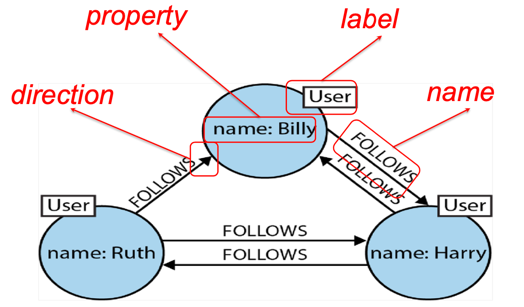
\includegraphics[width=0.5\columnwidth]{graphic/12-example-graph-store}

        \subsection{Graph Daten erzeugen}
        \begin{lstlisting}
                    CREATE (alice:User {username: 'Alice'}),
                           (bob:User {username: 'Bob'}),
                           (charlie:User {username: 'Charlie'}),
                           (alice)-[:ALIAS_OF]->(bob)

                    MATCH (bob:User {username:'Bob'}),
                          (charlie:User {username:'Charlie'}),
                          (davina:User {username:'Davina'}),
                          (edward:User {username:'Edward'})
                    CREATE (bob)-[:EMAILED]->(charlie),
                           (bob)-[:CC]->(davina),
                           (bob)-[:BCC]->(edward)
        \end{lstlisting}

        \subsection{Cypher Query Syntax}
        TODO: Einfügen aus Neo4J Cheat sheet

        \subsubsection{Example}
        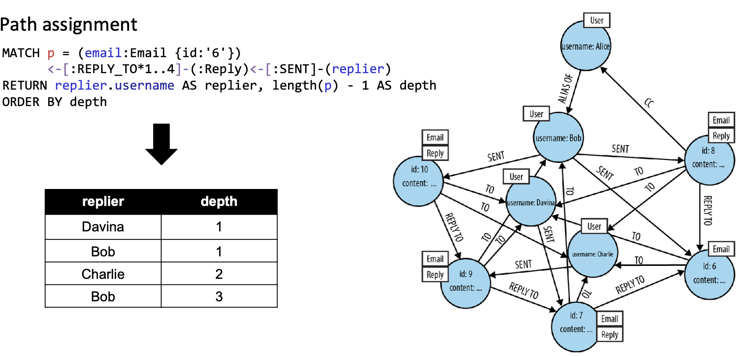
\includegraphics[width=\columnwidth]{graphic/13-example-cypher-query}
        
        \section{Column Family Stores {\tiny with Cassandra}}
        TODO: check if required

        \section{Column Stores}
        \begin{itemize}
            \item Massive DBs \enquote{read-mostly, read-intensive} (OLAP), DWH mit Sternschema
            \item Queries sind je nachdem schneller, Faktor 50 - 100, va. Aggregations-Fn. und Group By
        \end{itemize}
        \begin{tabularx}{\columnwidth}{X | X}
            \textbf{OLTP} & \textbf{OLAP} \\
            \textit{Online Transaction Processing} & \textit{Online Analytical Processing} \\
            \textit{Datenverwaltungs-optimiertes System} & \textit{Lese-Optimiertes System} \\
            \hline
            Low volume of data & High volume of data \\
            \hline
            High volume of transactions & Low volume of transactions \\
            \hline
            Typically normalized data & Typically denormalized data \\
            \hline
            ACID compliance & Not necessarily ACID-compliant \\
            \hline
            Require high availability & Doesn't usually require high availability
        \end{tabularx}

        \section{DuckDB - In-Process Analytical Column Store}
        TODO

        \section{Database-as-a-service (DbaaS)}
        Cloud-basierter Ansatz zur Speicherung und Verwaltung von strukturierten Daten.
        Cloud-DB-Dienste $\to$ als DbaaS zu klassifizieren

        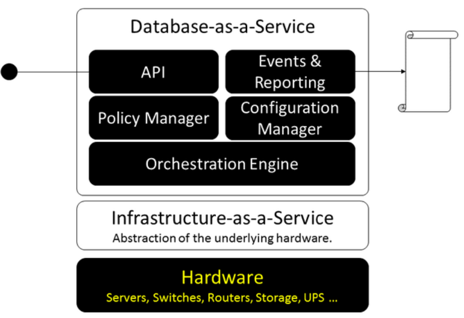
\includegraphics[scale=0.3]{graphic/14-dbaas-setup}

        \section{GraphQL}
        \begin{itemize}
            \item DB-API und REST Alternative
            \item Schema-basiert mit Typen
            \item Wickelt alle Anfragen über einzigen Endpoint ab
        \end{itemize}

        \subsection{Best Practices}
        \begin{enumerate}
            \item Nullable fields: Make fields non-nullable
            \item Miscommunication in the docs: GraphQL DocStrings (ähnlich Python)
            \item Lengthy arguments to mutations: Fasse zusammengehörige Attribute zu Type zusammen
            \item Insufficient mutation response
        \end{enumerate}

        \subsection{Schema Definition Language (SDL)}
        SDL ist DDL für GraphQL.
        \enquote{Scalar Types} sind Datentypen: Int (32-bit), Float (signed double-precision), String (UTF-8), Boolean.
        Weitere Typen sind: Enum, List, Union, Interface.

        \subsection{Postgraphile}
        \subsubsection{Schema / Types}
        Mit Tabelle \enquote{angestellter} macht Postgraphile folgendes (\enquote{by schema introspection/reflection}).
        \begin{tabularx}{\columnwidth}{X | X}
            \hline
            Types & \tabitem Type \enquote{Angestellter}, UpperCamelCase und singularized \\
            & \tabitem benennt Felder um in camelCase ohne \enquote{\_} \\
            & \tabitem ergänzt \texttt{nodeId} als Globally Unique Identifier falls PK existiert \\
            & \tabitem ergänzt Felder für jede Fremdschlüssel-Beziehung, z.B. \texttt{abteilungByAbtnr} \\
            \hline
            als Root \enquote{Query Types} & \tabitem Connection \enquote{allAngestellters} inkl. pagination, condition und order \\
            & \tabitem Felder für jeden Unique Constraint der Tabelle z.B. \texttt{angestellterByPersnr} \\
            \hline
            als Root \enquote{Mutation Types} & \tabitem \texttt{createAngestellter} \\
            & \tabitem \texttt{updateAngestellter} \\
            & \tabitem \texttt{deleteAngestellter}
        \end{tabularx}

        \subsubsection{Postgraphile Queries $\leftrightarrow$ SQL}
        \begin{lstlisting}
                    # PostGraphiQL
                    {
                        allAngestelltersList(first: 5, offset: 0) {
                            name
                            persnr
                            abtnr
                        }
                    }
                    # SQL
                    select name, persnr, abtnr from angestellter;

                    # -------------------------
                    # PostGraphiQL
                    query {
                        allAbteilungs {
                            edges {
                                node {
                                    abtnr
                                    name
                                }
                            }
                        }
                    }
                    # Returns
                    {
                        "data": {
                            "allAbteilungs": {
                                "edges": [
                                    {
                                        "node": {
                                            "abtnr": 1,
                                            "name": "Verkauf"
                                        }
                                    }, ...
                                ]
                            }
                        }
                    }
                    # SQL
                    select abtnr, name from abteilung;

                    # -------------------------
                    # PostGraphiQL
                    {
                        abteilungByAbtnr(abtnr: 1) {
                            abtnr
                            name
                        }
                    }
                    # Returns
                    {
                        "data": {
                            "abteilungByAbtnr": {
                                "abtnr": 1,
                                "name": "Verkauf"
                            }
                        }
                    }
                    # SQL
                    select abtnr, name from abteilung where abtnr = 1;
        \end{lstlisting}

        \subsubsection{Postgraphile Queries}
        \begin{lstlisting}
                    # query kann weggelassen werden:
                    query {
                        allAngestelltersList(first: 5, offset: 0) {
                            name
                            persnr
                            abtnr
                            chef
                        }
                    }
                    # gibt folgendes zurueck
                    {
                        "data": {
                        "allAngestelltersList": [
                            {
                                "name": "Marxer, Markus",
                                "persnr": 1001,
                                "abtnr": 1,
                                "chef": null
                            },
                            {
                                "name": "Widmer, Anna", ...
        \end{lstlisting}

        \begin{lstlisting}
                    query {
                        allAngestellters {
                            totalCount  # Info
                            pageInfo {  # Paginierung
                                startCursor
                                endCursor
                            }
                            nodes {
                                name ...
                            }
                        }
                    }
                    # gibt folgendes zurueck
                    {
                        "data": {
                            "allAngestellters": {
                                "totalCount": 23,
                                "pageInfo": {
                                    "startCursor": "WyJwcmltYXJ5X2tleV9hc...=",
                                    "endCursor": "WyJwcmltYXJ5X2tleV9hc2M...="
                                },
                            "nodes": [
                                ...
        \end{lstlisting}

        \subsubsection{Postgraphile Mutations}
        \begin{lstlisting}
                    mutation MyDeleteAbteilung99 {
                        deleteAbteilungByAbtnr(input: {abtnr: 99}) {
                            # clientMutationId
                            # deletedAbteilungId
                            abteilung {
                                abtnr
                                name
                            }
                        }
                    }
        \end{lstlisting}

        \section{Pagination}
        \begin{itemize}
            \item Durch Ergebnisse einer grossen Datenabfrage blättern
            \item Vorherige Seiten überspringen mit OFFSET
            \item OFFSET wird immer langsamer, je grösser
            \item erfordert eindeutige Sortierreihenfolge
            \item ist vom Client gesteuerte Eigenschaft der Verbindung
        \end{itemize}

        \subsection{Offset-Methode}
        \begin{lstlisting}[language=sql]
                    SELECT *
                    FROM customers
                    ORDER BY customerid
                    OFFSET 100000 FETCH NEXT 25 ROWS ONLY
                    -- einfach, verbreitet, aber skaliert nicht
        \end{lstlisting}

        \subsection{Seek-Methode}
        \begin{lstlisting}[language=sql]
                    -- index gegeben
                    CREATE INDEX customers_pkey_idx ON customers (customerId);

                    SELECT *
                    FROM customers
                    WHERE customerid > 100000
                    ORDER BY customerid
                    FETCH NEXT 25 ROWS ONLY
                    -- anstelle von wert 100000 kann auch cursor treten
                    -- effizienter als offset-methode
        \end{lstlisting}



        \section{Database Design Patterns}
        \subsection{Data Mapper}
        \begin{itemize}
            \item CRUD-Funktionen auf Objekten (in DB persistent)
            \item Bildet Entität in DB ab
            \item Implementiert durch OR/Mapper
        \end{itemize}

        \subsection{Active Record}
        \begin{itemize}
            \item Speichert Daten in relationaler Datenbank
            \item \enquote{One Object - One Record}
        \end{itemize}

        \subsection{CQRS {\tiny Command-Query Responsibility Segregation}}
        \begin{itemize}
            \item Geeignet für: Real-time analytics, viele Schreibprozesse (>1:100), verteilte Systeme, No-Schema-Approach
            \item Trennt Domänenmodell in Read-Modell und Write-Modell (bzw. Query und Command)
            \item Schreiben und Abfragen wird separat behandelt, Optimierung beider Befehle
            \item Probleme
            \subitem Unnötige Komplexität
            \subitem Aufwändige Koordination
            \subitem Star Schema und Snowflake Schema könnte man als CQRS bezeichnen
        \end{itemize}
        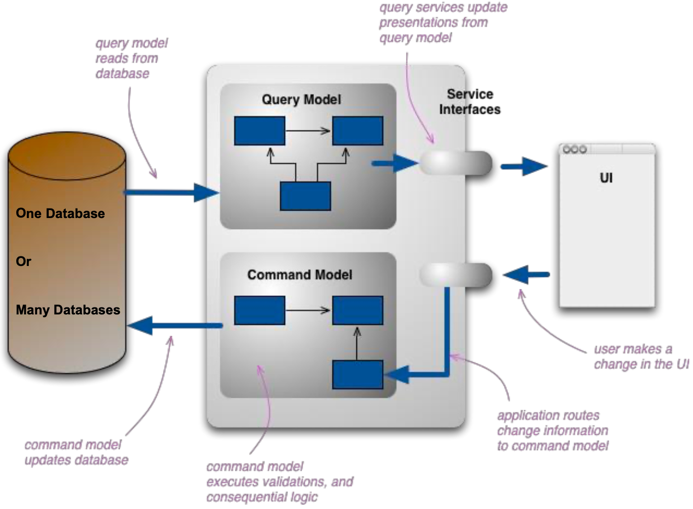
\includegraphics[width=\columnwidth]{graphic/11-cqrs-modell}

        \subsection{Event Sourcing}
        \enquote{Turning the database inside-out}
        \begin{itemize}
            \item Reihe von Änderungen (Events) im Zustand einer Anwendung
            \item Events sind unveränderlich (\enquote{append-only})
            \item Events werden als Stornotransaktionen eingefügt, nicht gelöscht
            \item Event Sourcing unabhängig von CQRS, aber oft in Kombination
        \end{itemize}

        \subsection{Evolutionary Database Design}
        TODO

    \end{multicols*}
\end{document}